\documentclass{article}
\usepackage{graphicx}
\begin{document}
\section*{First Python program - doing calculations}
\texttt{xkcd} is a ``\emph{webcomic about romance, sarcasm, math and language}''. 
Every now and then, you'll find a gem like this: \newline
\begin{figure}[h]
\begin{center}
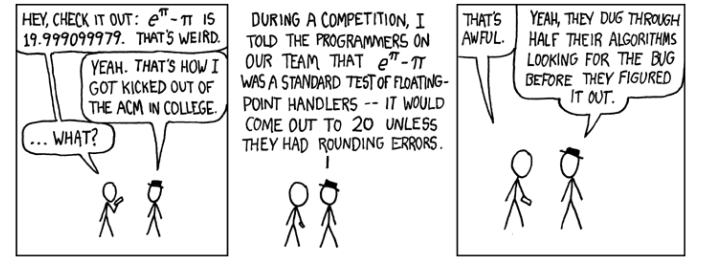
\includegraphics[height=130pt]{../pictures/xkcd_pi.png}
\emph{Also, I hear the 4th root of (9\^{}2 + 19\^{}2/22) is pi.}
\end{center}
\end{figure}

Verify the above claims by running the calculations on a Python shell. Also, write a 
Python script that does the same. Your script should print out the values when it is
run.
\end{document}
